\documentclass[letterpaper]{article} % DO NOT CHANGE THIS
\usepackage[submission]{aaai2027}  % DO NOT CHANGE THIS
\usepackage[hyphens]{url}  % DO NOT CHANGE THIS
\usepackage{graphicx} % DO NOT CHANGE THIS
\urlstyle{rm} % DO NOT CHANGE THIS
\def\UrlFont{\rm}  % DO NOT CHANGE THIS
\usepackage{natbib}  % DO NOT CHANGE THIS AND DO NOT ADD ANY OPTIONS TO IT
\usepackage{caption} % DO NOT CHANGE THIS AND DO NOT ADD ANY OPTIONS TO IT
\frenchspacing  % DO NOT CHANGE THIS

\usepackage{algorithm}
\usepackage{algorithmic}

\usepackage{booktabs}
\usepackage{amsmath, amssymb}

\usepackage{tikz}
\usetikzlibrary{arrows.meta, positioning, calc, shapes.geometric}

%
% Keep the \pdfinfo as shown here. There's no need
% for you to add the /Title and /Author tags.
\pdfinfo{
/TemplateVersion (2027.1)
}

\setcounter{secnumdepth}{0}

% ── Figure colours (figures only; no colour in text) ─────────────────────────
\definecolor{figblue}{RGB}{30,70,120}
\definecolor{figorange}{RGB}{247,127,0}
\definecolor{figgreen}{RGB}{76,175,80}
\definecolor{figred}{RGB}{214,40,40}
\definecolor{figpurple}{RGB}{120,50,160}

% ── TikZ styles shared by the figures ────────────────────────────────────────
\tikzset{
  bxL/.style={draw=figorange!80!black, fill=figorange!15, rounded corners=3pt,
              minimum width=#1, minimum height=0.85cm, align=center,
              font=\small, line width=0.8pt},
  bxC/.style={draw=gray!70, fill=gray!10, rounded corners=3pt,
              minimum width=#1, minimum height=0.85cm, align=center,
              font=\small, line width=0.8pt},
  arr/.style={-{Stealth[length=5pt]}, thick},
  cnode/.style={circle, draw=figblue, fill=figblue!20,
                minimum size=0.45cm, inner sep=0pt, font=\footnotesize},
  fvec/.style={draw=figpurple!70!black, fill=figpurple!10, rounded corners=2pt,
               minimum width=0.9cm, minimum height=0.5cm, font=\footnotesize},
  mlp/.style={draw=figorange!80!black, fill=figorange!20, rounded corners=2pt,
              minimum width=0.9cm, minimum height=0.55cm, font=\footnotesize},
  score/.style={draw=figgreen!60!black, fill=figgreen!15, rounded corners=2pt,
                minimum width=0.9cm, minimum height=0.45cm, font=\footnotesize},
}

\title{Learning-Guided Simulated Annealing for the Capacitated Vehicle Routing Problem}
\author{
    Anonymous Submission
}
\affiliations{
}

\begin{document}

\maketitle

\begin{abstract}
% TODO: Abstract to be written last.
\end{abstract}

% ============================================================================
\section{Introduction}
% ============================================================================
% TODO: Introduction.
% Suggested flow (from the slides / old draft):
%   - CVRP: fundamental NP-hard problem, practical relevance.
%   - Improvement metaheuristics (SA): robust, handle capacity constraints
%     naturally, but propose moves blindly -> slow convergence.
%   - Neural combinatorial optimization: construction vs improvement methods;
%     improvement learners are powerful but heavyweight at inference.
%   - Our idea: keep the SA skeleton, replace only the blind proposal with a
%     tiny learned policy (extends Neural SA [Correia et al. 2023] to CVRP).
%   - Contributions bullet list.
%   - Paper organization paragraph.

% ============================================================================
\section{Background and Related Work}
% ============================================================================
% TODO: Related work.
% Suggested coverage: exact methods and classical heuristics/metaheuristics
% (Clarke-Wright, 2-opt, SA, OR-Tools, LKH/HGS); neural construction methods
% (Nazari, Kool AM, POMO); neural improvement methods (Wu, DACT, NLNS, CDCP,
% IIL); Neural Simulated Annealing (Correia et al. 2023) and why extending it
% to CVRP is non-trivial (capacity constraints, feasibility).

% ============================================================================
\section{Problem Definition}
\label{sec:problem_definition}
% ============================================================================

The \textit{Capacitated Vehicle Routing Problem (CVRP)} is defined on a complete undirected graph $G = (V, E)$, where $V = \{0\} \cup \mathcal{C}$ and $E = V \times V$ denote the sets of nodes and edges, respectively. Node $0$ corresponds to the central depot, and $\mathcal{C} = \{1, \dots, N\}$ represents the set of $N$ customers.

Each edge $(i, j) \in E$ is associated with a travel cost $c_{ij} = \|\mathbf{p}_i - \mathbf{p}_j\|_2$, the Euclidean distance between the 2D coordinates $\mathbf{p}_i, \mathbf{p}_j \in [0,1]^2$, satisfying $c_{ij} = c_{ji}$. Each customer $i \in \mathcal{C}$ has a non-negative demand $q_i$, while the depot has zero demand ($q_0 = 0$). An unlimited fleet of identical vehicles, each with uniform capacity $Q$, is stationed at the depot; the number of routes $m$ is therefore a decision variable unconstrained from above.

A route $R_k = (0, v_1, v_2, \ldots, v_p, 0)$ is a simple cycle starting and ending at the depot, where $\{v_1, \ldots, v_p\} \subseteq \mathcal{C}$ denotes the subset of customers served by vehicle $k$. A \textit{solution} $s = \{R_1, \ldots, R_m\}$ consists of a set of $m$ routes. A solution $s$ is \textit{feasible} if and only if it satisfies the following conditions:
\begin{enumerate}
    \item Each customer is visited exactly once by a single vehicle,
    $$
    \sum_{k=1}^{m} \mathbf{1}_{\{i \in R_k\}} = 1, \quad \forall i \in \mathcal{C} .
    $$
    \item For every route $R_k$, the total demand of its customers does not exceed the vehicle capacity $Q$, i.e.,
    $$
    \sum_{i \in R_k \setminus \{0\}} q_i \leq Q, \quad \forall k = 1, \ldots, m.
    $$
\end{enumerate}
The set of \textit{feasible solutions} is denoted by $\mathcal{F}$.

Let $x_{ij}(s)$ be a binary indicator variable with $x_{ij}(s) = 1$ if edge $(i,j)$ is traversed in any route $R_k$ of $s$, and $x_{ij}(s) = 0$ otherwise. The objective of the CVRP is to find a feasible solution $s^* \in \mathcal{F}$ that minimizes the total travel cost $C(s)$:
$$
s^* = \arg\min_{s \in \mathcal{F}} \Big\{ C(s) = \sum_{i \in V} \sum_{j \in V,\, i < j} c_{ij}\, x_{ij}(s) \Big\}.
$$

% ============================================================================
\section{Proposed Method}
% ============================================================================

\subsection{Overview}

We propose \emph{Learning-Guided Simulated Annealing} (LG-SA), a hybrid method that combines \textit{Simulated Annealing} (SA) with a lightweight neural policy trained by \textit{Reinforcement Learning} (RL). Following the Neural Simulated Annealing framework \citep{correia_neural_2023}, the SA component orchestrates the global exploration of the solution space through its acceptance criterion and cooling schedule, while the neural network replaces the single blind component of SA --- the uniform move proposal --- with a learned, state-dependent proposal distribution. This design contrasts with ``heavyweight'' improvement architectures such as the Dual-Aspect Collaborative Transformer \citep{ma_learning_2021}, which replace the heuristic logic entirely with a deep encoder: our policy remains deliberately small, so that the guided search retains a per-step cost close to that of classical SA and can be batched over thousands of instances on a single GPU.

\textit{Simulated Annealing} \citep{kirkpatrick_optimization_1983} iteratively explores the neighborhood of a current solution. Given a solution $s$, SA samples a neighboring solution $s' \in \mathcal{N}(s)$ and accepts it according to the \textit{Metropolis criterion}: improving moves are always accepted, while worsening moves are accepted with probability $\exp(-\Delta C / T)$, where $\Delta C = C(s') - C(s)$ is the cost difference and $T$ the current temperature. The temperature decays from an initial value $T_0$ to a final value $T_{\mathrm{final}}$ over the search horizon according to a monotone cooling schedule, which regulates the transition from exploration to exploitation.

Neighboring solutions are produced by a \textit{neighborhood operator} $H: \mathcal{S} \times \mathcal{A} \to \mathcal{S}$ that maps a solution $s$ and an action $a \in \mathcal{A}(s)$ to the neighbor $s' = H(s, a)$, so that
$$
\mathcal{N}(s) = \left\{ H(s, a) : a \in \mathcal{A}(s) \right\}.
$$
In our setting, an action designates a pair of nodes $a = (i, j)$, and $H$ applies a standard pairwise local search move to them (e.g., relocating node $i$ next to node $j$). The operator is a modular component of the framework; the candidate operators and their comparison are presented in the experimental section.

Whereas classical SA draws $a$ uniformly over $\mathcal{A}(s)$, LG-SA samples it from a policy $\pi_\theta$ conditioned on the current solution:
\begin{equation*}
a \sim \pi_\theta(\cdot \mid s) \quad \text{ and } \quad s' = H(s, a) \in \mathcal{N}(s).
\end{equation*}
Everything else --- the operator, the Metropolis acceptance, the cooling schedule --- is kept from classical SA. The overall procedure is summarized in Algorithm~\ref{alg:lgsa} and illustrated in Figure~\ref{fig:pipeline}.

\begin{figure*}[t]
\centering
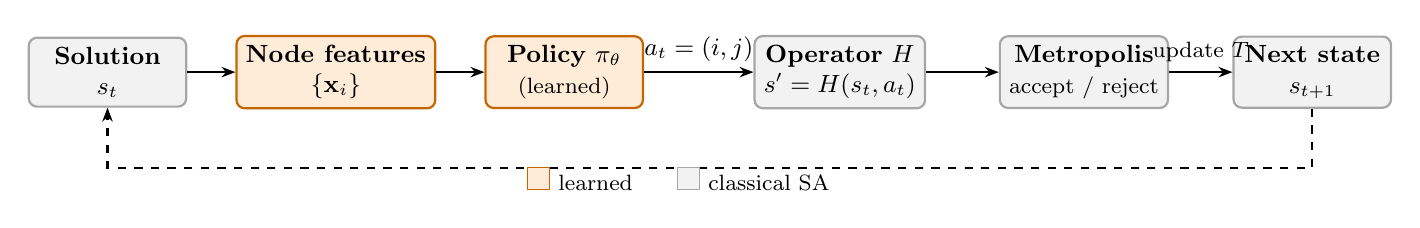
\begin{tikzpicture}[>=Stealth, thick]
  \node[bxC=2.0cm] (s)    at (0,0)    {\textbf{Solution}\\$s_t$};
  \node[bxL=2.0cm] (feat) at (2.9,0)  {\textbf{Node features}\\$\{\mathbf{x}_i\}$};
  \node[bxL=2.0cm] (pi)   at (5.8,0)  {\textbf{Policy} $\pi_\theta$\\{\footnotesize (learned)}};
  \node[bxC=2.0cm] (H)    at (9.3,0)  {\textbf{Operator} $H$\\$s' = H(s_t, a_t)$};
  \node[bxC=2.0cm] (M)    at (12.4,0) {\textbf{Metropolis}\\{\footnotesize accept / reject}};
  \node[bxC=2.0cm] (sn)   at (15.3,0) {\textbf{Next state}\\$s_{t+1}$};

  \draw[arr] (s)    -- (feat);
  \draw[arr] (feat) -- (pi);
  \draw[arr] (pi)   -- node[midway, above, font=\small] {$a_t = (i,j)$} (H);
  \draw[arr] (H)    -- (M);
  \draw[arr] (M)    -- node[midway, above, font=\footnotesize] {update $T$} (sn);
  \draw[arr, dashed] (sn.south) -- ++(0,-0.75) -| (s.south);

  \node[font=\footnotesize, anchor=west] at (5.2,-1.35)
    {\tikz{\fill[figorange!15, draw=figorange!80!black, line width=0.6pt] (0,0) rectangle (0.28,0.28);}~learned
     \hspace{1.2em}
     \tikz{\fill[gray!10, draw=gray!70, line width=0.6pt] (0,0) rectangle (0.28,0.28);}~classical SA};
\end{tikzpicture}
\caption{The LG-SA loop. Classical SA components (gray) are kept unchanged: the operator $H$, the Metropolis acceptance, and the cooling schedule. The only modified block is the move proposal (orange): the current solution is encoded into per-node feature vectors and a learned policy samples the node pair $a_t = (i,j)$, replacing the uniform sampling of classical SA.}
\label{fig:pipeline}
\end{figure*}

\begin{algorithm}[tb]
\caption{Learning-Guided Simulated Annealing}
\label{alg:lgsa}
\textbf{Input}: instance, initial solution $s$, policy $\pi_\theta$, operator $H$\\
\textbf{Output}: best solution found $s^*$
\begin{algorithmic}[1]
\STATE Initialize $s^* \gets s$ and temperature $T \gets T_0$
\WHILE{termination criterion not met}
\STATE Encode $s$ into per-node feature vectors
\STATE Sample action $a \sim \pi_\theta(\cdot \mid s)$ \hfill (guided proposal)
\STATE Generate candidate $s' \gets H(s, a)$
\STATE $s \gets s'$ with probability $\min\!\left(1, e^{-\Delta C / T}\right)$ \hfill (Metropolis)
\STATE Update $s^*$ if $C(s) < C(s^*)$; cool $T$
\ENDWHILE
\STATE \textbf{return} $s^*$
\end{algorithmic}
\end{algorithm}

\subsection{The Guided Search as a Markov Decision Process}

To learn the proposal distribution with RL, we frame the SA loop as a Markov Decision Process. At step $t$, the \textit{state} $s_t$ is the current feasible solution together with the search meta-information (current temperature and remaining budget), encoded as a set of per-node feature vectors described below. The \textit{action} $a_t = (i, j)$ is the node pair handed to the operator $H$. The \textit{transition} is the composition of the operator and the stochastic Metropolis acceptance: the next state is $H(s_t, a_t)$ if the move is accepted and $s_t$ otherwise, so the environment dynamics include the acceptance randomness of SA.

The \textit{reward} is derived from the evolution of the solution cost along the search: a move that is accepted and improves the solution receives a positive reward proportional to the (normalized) cost reduction, a rejected move yields no improvement signal, and proposals leading to infeasible neighbors can be penalized. Reward variants that instead emphasize improvements of the best solution found so far, or the final solution quality at the end of the horizon, fit the same framework; the precise shaping is a design choice studied experimentally. The agent thus maximizes the expected cumulative discounted reward over the SA horizon, which aligns the learned proposal with the overall goal of driving the annealing process toward low-cost solutions rather than with any single greedy step.

\subsection{Node-Centric State Representation}

To be applicable to any problem size $N$ and to remain \textit{scale-invariant}, the state is encoded in a \textit{node-centric} fashion: each node $i$ carries its own local feature vector $\mathbf{x}_i$, and no fixed-size global descriptor is used. The features fall into four groups:
\begin{itemize}
    \item \textit{Static instance features:} node coordinates, polar coordinates relative to the depot, a depot indicator, and the normalized demand $q_i / Q$;
    \item \textit{Solution topology and local geometry:} the coordinates of the node's current predecessor and successor in its route, together with local quality signals such as the detour cost incurred by the node at its current position, its distance to the route centroid, and local density statistics of the instance;
    \item \textit{Capacity status:} the load ratio and remaining slack of the node's current route, and the node's own contribution to that load;
    \item \textit{Search meta-features:} the current (normalized) SA temperature and the fraction of the search budget remaining, which let the policy adapt its behavior to the phase of the annealing schedule.
\end{itemize}
All features are local to a node and standardized, so the same trained model can be deployed on instances of arbitrary size without retraining. The complete list of features, with their formal definitions, is given in the appendix; their individual contribution is analyzed in the experimental section.

\subsection{Two-Stage Conditional Policy}
\label{sec:policy}

\begin{figure*}[t]
\centering
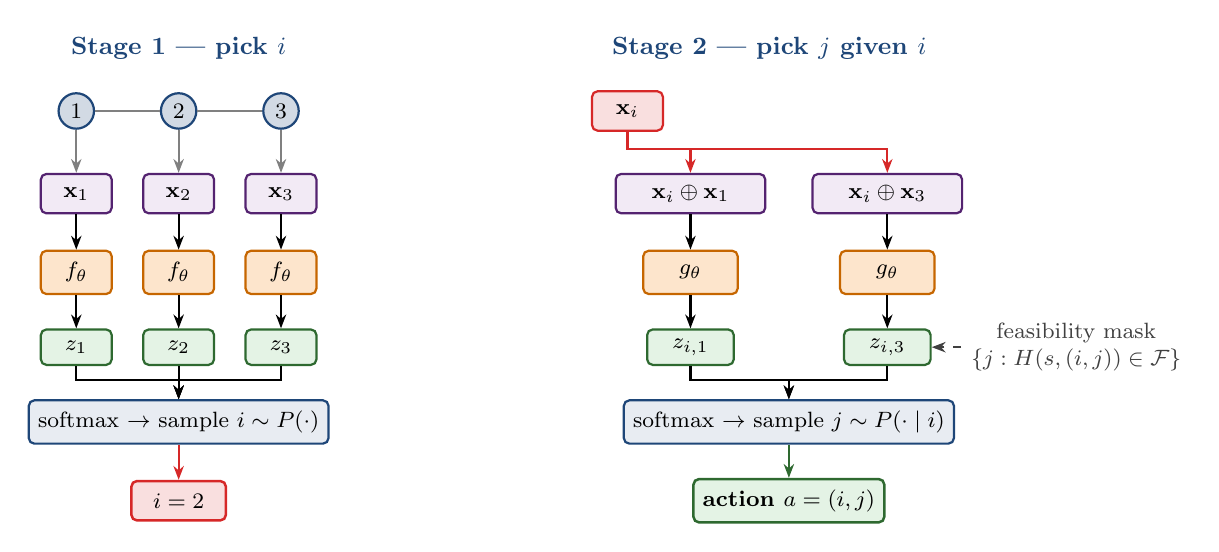
\begin{tikzpicture}[>=Stealth, thick]

  % ─── Stage 1 (left): score every node ──────────────────────────────
  \node[font=\small\bfseries, figblue] at (0.6, 3.0) {Stage 1 --- pick $i$};

  % CVRP fragment (3 nodes in a route)
  \node[cnode] (n1) at (-0.7, 2.2) {1};
  \node[cnode] (n2) at (0.6,  2.2) {2};
  \node[cnode] (n3) at (1.9,  2.2) {3};
  \draw[gray, thick] (n1) -- (n2) -- (n3);

  % Feature vectors
  \node[fvec] (x1) at (-0.7, 1.15) {$\mathbf{x}_1$};
  \node[fvec] (x2) at (0.6,  1.15) {$\mathbf{x}_2$};
  \node[fvec] (x3) at (1.9,  1.15) {$\mathbf{x}_3$};
  \draw[arr, gray] (n1) -- (x1);
  \draw[arr, gray] (n2) -- (x2);
  \draw[arr, gray] (n3) -- (x3);

  % Shared MLP
  \node[mlp] (m1a) at (-0.7, 0.15) {$f_\theta$};
  \node[mlp] (m1b) at (0.6,  0.15) {$f_\theta$};
  \node[mlp] (m1c) at (1.9,  0.15) {$f_\theta$};
  \draw[arr] (x1) -- (m1a);
  \draw[arr] (x2) -- (m1b);
  \draw[arr] (x3) -- (m1c);

  % Scores
  \node[score] (z1) at (-0.7, -0.8) {$z_1$};
  \node[score] (z2) at (0.6,  -0.8) {$z_2$};
  \node[score] (z3) at (1.9,  -0.8) {$z_3$};
  \draw[arr] (m1a) -- (z1);
  \draw[arr] (m1b) -- (z2);
  \draw[arr] (m1c) -- (z3);

  % Softmax + sample
  \node[draw=figblue, fill=figblue!10, rounded corners=2pt,
        minimum width=3.4cm, minimum height=0.55cm, font=\footnotesize]
    (s1) at (0.6, -1.75) {softmax $\to$ sample $i \sim P(\cdot)$};
  \draw[arr] (z1.south) -- ++(0,-0.18) -| (s1.north);
  \draw[arr] (z2) -- (s1);
  \draw[arr] (z3.south) -- ++(0,-0.18) -| (s1.north);

  % Highlight chosen i (say i = 2)
  \node[draw=figred, fill=figred!15, rounded corners=2pt, line width=0.9pt,
        minimum width=1.2cm, minimum height=0.5cm, font=\footnotesize\bfseries]
    (chosen) at (0.6, -2.75) {$i = 2$};
  \draw[arr, figred] (s1) -- (chosen);

  % ─── Stage 2 (right): pick j given i ───────────────────────────────
  \node[font=\small\bfseries, figblue] at (8.1, 3.0) {Stage 2 --- pick $j$ given $i$};

  % Carry over x_i (selected)
  \node[fvec, fill=figred!15, draw=figred] (xi) at (6.3, 2.2) {$\mathbf{x}_i$};

  % Pair concatenations (with the two other nodes)
  \node[fvec, minimum width=1.9cm] (c1) at (7.1, 1.15) {$\mathbf{x}_i \oplus \mathbf{x}_1$};
  \node[fvec, minimum width=1.9cm] (c3) at (9.6, 1.15) {$\mathbf{x}_i \oplus \mathbf{x}_3$};

  \draw[arr, figred] (xi.south) -- ++(0,-0.22) -| (c1.north);
  \draw[arr, figred] (xi.south) -- ++(0,-0.22) -| (c3.north);

  % MLP2
  \node[mlp, minimum width=1.2cm] (m2a) at (7.1, 0.15) {$g_\theta$};
  \node[mlp, minimum width=1.2cm] (m2b) at (9.6, 0.15) {$g_\theta$};
  \draw[arr] (c1) -- (m2a);
  \draw[arr] (c3) -- (m2b);

  % Pair scores + feasibility mask
  \node[score, minimum width=1.1cm] (zi1) at (7.1, -0.8) {$z_{i,1}$};
  \node[score, minimum width=1.1cm] (zi3) at (9.6, -0.8) {$z_{i,3}$};
  \draw[arr] (m2a) -- (zi1);
  \draw[arr] (m2b) -- (zi3);

  \node[font=\footnotesize, align=center, gray!50!black] (maskbox) at (12.0, -0.8)
    {feasibility mask\\$\{j : H(s,(i,j)) \in \mathcal{F}\}$};
  \draw[arr, gray!50!black, dashed] (maskbox.west) -- (zi3.east);

  % Softmax + sample j
  \node[draw=figblue, fill=figblue!10, rounded corners=2pt,
        minimum width=3.8cm, minimum height=0.55cm, font=\footnotesize]
    (s2) at (8.35, -1.75) {softmax $\to$ sample $j \sim P(\cdot \mid i)$};
  \draw[arr] (zi1.south) -- ++(0,-0.18) -| (s2.north);
  \draw[arr] (zi3.south) -- ++(0,-0.18) -| (s2.north);

  % Final action
  \node[draw=figgreen!60!black, fill=figgreen!15, rounded corners=2pt, line width=0.9pt,
        minimum width=2.2cm, minimum height=0.55cm, font=\footnotesize\bfseries]
    (act) at (8.35, -2.75) {action $a = (i,j)$};
  \draw[arr, figgreen!60!black] (s2) -- (act);

\end{tikzpicture}
\caption{Two-stage conditional sampling of the node pair $(i,j)$, shown on a toy route of three customers. Stage 1: every node's feature vector is scored independently by a shared network $f_\theta$ and the first node $i$ is sampled from the softmax over the scores. Stage 2: the representation of the selected node $i$ is combined with that of every candidate partner $j$ and scored by a second network $g_\theta$; infeasible partners are masked out before the softmax, and $j$ is sampled from the conditional distribution. The factorization $P(i,j) = P(i) \cdot P(j \mid i)$ makes each proposal $\mathcal{O}(N)$.}
\label{fig:twostage}
\end{figure*}

The policy must define a distribution over the $\mathcal{O}(N^2)$ node pairs while remaining cheap enough to be evaluated at every SA step. We therefore factorize the joint selection as
$$
P(i, j \mid s) = P(i \mid s) \cdot P(j \mid i, s),
$$
and implement it with a lightweight two-stage architecture, illustrated in Figure~\ref{fig:twostage}. In the first stage, a small network $f_\theta$ maps each feature vector to a scalar score $z_i = f_\theta(\mathbf{x}_i)$, and the first node is sampled from the softmax distribution over these scores:
$$
i \sim P(\cdot \mid s) = \mathrm{softmax}\big( \{ z_i : i \in \mathcal{C} \} \big).
$$
In the second stage, the representation of the selected node $i$ is combined with that of every other node $j$, and a second network $g_\theta$ assigns a conditional score $z_{ij} = g_\theta(\mathbf{x}_i, \mathbf{x}_j)$ from which the partner is sampled:
$$
j \sim P(\cdot \mid i, s) = \mathrm{softmax}\big( \{ z_{ij} : j \in \mathcal{C} \} \big).
$$
Both stages are built from small multilayer perceptrons applied identically to every node, which makes the policy permutation-equivariant. The second stage can additionally be conditioned on cheap pairwise descriptors of the candidate move (e.g., the exact cost of the move joining $i$ and $j$), computed only for the selected $i$.

This factorization also provides a natural hook for the capacity constraints: once $i$ is selected, the partners $j$ for which $H(s, (i,j))$ would be infeasible are masked out of the second-stage distribution, so every proposed neighbor is feasible at the price of $\mathcal{O}(N)$ feasibility checks per step. Alternative constraint-handling strategies are discussed and compared in the experimental section.

Since the conditional network is evaluated only for the single selected first node, each proposal costs $\mathcal{O}(N)$ --- as opposed to the $\mathcal{O}(N^2)$ cost of scoring all pairs jointly --- and the whole step is expressed as batched tensor operations, allowing thousands of instances to be advanced in parallel on one GPU.

\subsection{Training with PPO}
\label{sec:training}

The policy is trained with \textit{Proximal Policy Optimization} (PPO) \citep{schulman_proximal_2017}, the standard on-policy actor-critic algorithm. Training alternates between a \textit{collection} phase, in which the current policy runs the full LG-SA loop of Algorithm~\ref{alg:lgsa} on a large batch of freshly generated instances in parallel and stores every transition $(s_t, a_t, r_t)$, and an \textit{update} phase, in which the stored episodes are replayed for several optimization epochs. Advantages are estimated with Generalized Advantage Estimation, and the actor maximizes the usual clipped surrogate objective with an entropy bonus; we refer to \citet{schulman_proximal_2017} for the standard formulation and only detail our departures from it.

The critic $V_\phi$ is a separate permutation-invariant network: it encodes each node feature vector independently, pools the embeddings across nodes into a fixed-size summary, and maps this summary to a scalar value estimate. Keeping the actor and critic distinct prevents interference between the policy and value representations.

Our implementation departs from standard PPO in three ways, all aimed at stabilizing training on the long and noisy SA horizon:
\begin{itemize}
    \item \textit{Hybrid clipping--KL objective.} Rather than choosing between the clipped surrogate and the KL-penalized objective, we use both: an adaptive Kullback--Leibler penalty $\beta_{\text{KL}}\, D_{\text{KL}}(\pi_{\theta_{\text{old}}} \| \pi_\theta)$ is added to the clipped loss, and its coefficient is doubled or halved after each update epoch depending on whether the measured divergence leaves a band around a target value. This soft trust region allows many optimization epochs on each collected batch without catastrophic policy drift.
    \item \textit{KL-coupled learning rate.} The same divergence signal modulates the actor's learning rate within fixed bounds --- gently decreased when the policy moves too fast, increased when it stalls --- so the effective step size tracks the trust region automatically.
    \item \textit{Regularized critic.} The value loss is clipped, mirroring the actor's trust region, and augmented with a gradient penalty that encourages a smooth (near-Lipschitz) value landscape; we found this useful given that consecutive states differ by a single local move whose acceptance is itself stochastic.
\end{itemize}

% ============================================================================
\section{Experimental Results}
\label{sec:experiments}
% ============================================================================

\subsection{Experimental Setup}
% TODO: benchmarks (Nazari uniform test set, CVRPLIB Set X / Uchoa,
% Queiroga Set XML), hardware, training protocol, stability analysis,
% baselines (LKH3, OR-Tools, neural construction and improvement methods).

\subsection{Local Search Operators and Feasibility Strategies}
% TODO: cross-evaluation of {insertion, swap, 2-opt} x {proactive, reactive,
% indirect}; adopted configuration.
%
% --- Material moved from the method section (operators) -------------------
% We consider three standard neighborhood operators defined over a pair of
% nodes (i, j). The operator is fixed for a given model: the policy is
% trained to propose moves for one operator.
% \begin{itemize}
%     \item \textit{Swap:} exchanges the positions of nodes $i$ and $j$,
%           within a route or across routes;
%     \item \textit{Insertion (relocation):} removes node $i$ from its
%           current position and reinserts it immediately after node $j$;
%     \item \textit{2-opt / 2-opt*:} reverses the path segment between $i$
%           and $j$ for intra-route moves, and exchanges the route suffixes
%           following $i$ and $j$ for inter-route moves.
% \end{itemize}
%
% --- Material moved from the method section (feasibility strategies) ------
% Under capacity constraints, many actions produce an infeasible neighbor
% $H(s,a) \notin \mathcal{F}$, which is the central obstacle in extending
% neural SA from unconstrained problems to the CVRP. We consider three
% strategies to keep the search within $\mathcal{F}$.
%
% \paragraph{Proactive feasibility filtering (action masking).}
% Let $\mathcal{A}_f(s) = \{ a \in \mathcal{A}(s) : H(s, a) \in \mathcal{F} \}$
% denote the feasible action subset. The policy is restricted to it by
% masking infeasible actions with zero probability before sampling. This
% strategy exploits the conditional factorization of the policy: the first
% node $i$ is selected freely, and only then are the feasible partners
% $\{ j : H(s, (i,j)) \in \mathcal{F} \}$ computed and used to mask the
% second stage. Feasibility therefore requires only $\mathcal{O}(N)$ checks
% per step instead of $\mathcal{O}(N^2)$. Every proposed neighbor is feasible
% by construction; since the fleet is unlimited, a node can always open a new
% route, so the feasible set is never empty.
%
% \paragraph{Reactive rejection.}
% The policy samples any action from its learned distribution, and the
% resulting neighbor is checked afterwards: if $s' \notin \mathcal{F}$, the
% move is rejected and the current solution is retained. This avoids the
% overhead of explicit filtering but can waste both compute and learning
% signal when many sampled moves are infeasible.
%
% \paragraph{Indirect representation with greedy reconstruction.}
% Feasibility can be delegated to the representation itself: the solution is
% encoded as an unconstrained permutation of the customers, the policy
% modifies the permutation, and a deterministic \textit{greedy split}
% heuristic packs the permutation back into capacity-feasible routes
% \citep{vidal_technical_2016}. Every state is feasible by construction and
% the policy never handles constraints, but the reconstruction runs at every
% search step and its cost grows with the problem size.
% ---------------------------------------------------------------------------

\subsection{Ablation Studies}
% TODO: feature ablations (LOO, thematic, isolation), reward formulations,
% network size, Metropolis on/off, greedy vs sampling, initialization,
% curriculum depth.
%
% --- Material moved from the method section (stochastic inference) --------
% \paragraph{Stochastic proposals at inference.}
% In standard RL applications, trained policies are often exploited greedily
% by selecting the most probable action. Our framework deviates from this
% practice: since the policy acts as the proposal distribution of an SA step,
% we retain stochastic sampling, $a_t \sim \pi_\theta(\cdot \mid s_t)$, at
% inference as well. A greedy policy would repeatedly propose the same
% ``best'' move, collapsing the diversity that the Metropolis criterion needs
% to balance exploration and exploitation; sampling from the full
% distribution provides SA with a stream of varied, high-quality candidates.
%
% --- Material moved from the method section (diverse initializations) -----
% \paragraph{Diverse initializations.}
% Each training episode starts from an initial solution produced by a
% constructive heuristic drawn from a pool (random assignment, nearest
% neighbor, sweep, and single-customer routes). Mixing initializations
% exposes the policy to qualitatively different regions of the solution space
% and prevents it from overfitting to the basin of a single construction
% heuristic; the pool can be introduced progressively over training.
%
% --- Material moved from the method section (curriculum) ------------------
% \paragraph{Curriculum over the search horizon.}
% Training episodes are much shorter than the search budgets used at
% deployment. To expose the policy to the later, fine-grained phase of the
% search --- states near local optima that a short episode started from a raw
% construction rarely reaches --- we use a curriculum on the starting point:
% before collection, each batch of instances is first \textit{warmed up} by
% the current policy for a number of steps that grows over the course of
% training according to a monotone schedule. Early in training the policy
% thus learns to repair poor solutions, and later it increasingly learns to
% improve already-refined ones. Optionally, each instance is warmed to its
% own randomly drawn depth, so that a single batch covers the entire spectrum
% from raw initializations to deeply improved solutions.
% ---------------------------------------------------------------------------

\subsection{Comparison with Baselines}
% TODO: main results table at N=100 (cost / time vs classical and neural
% baselines), guided vs blind SA curves.

\subsection{Generalization and Scalability}
% TODO: cross-distribution generalization, larger N without retraining,
% runtime scaling.

% ============================================================================
\section{Conclusion}
% ============================================================================
% TODO: Conclusion and future work (LNS operators, GNN encoders, richer VRP
% variants).

% ============================================================================
\appendix
\section{Appendix: State Feature Definitions}
\label{app:features}
% ============================================================================

This appendix defines every component of the node feature vector $\mathbf{x}_i$ used by the policy and the critic. Throughout, $\mathrm{prev}(i)$ and $\mathrm{succ}(i)$ denote the nodes immediately before and after $i$ in the current visiting order, $r(i)$ the route currently serving $i$, $Q_{r(i)}$ the total load of that route, and $d(\cdot, \cdot)$ the Euclidean distance. Figure~\ref{fig:features} illustrates the geometric quantities. All features are normalized to comparable ranges, and each is computed locally at node $i$: the encoding contains no fixed-size global descriptor, which is what makes the representation applicable to any instance size.

\begin{figure}[t]
\centering
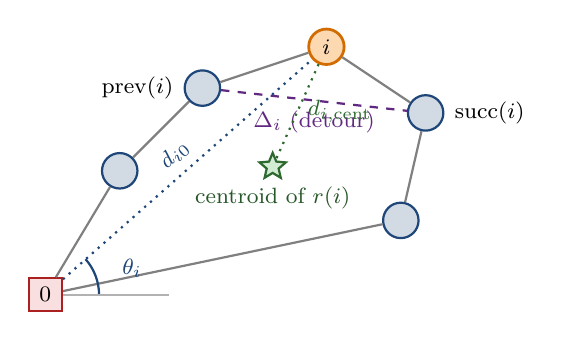
\begin{tikzpicture}[>=Stealth, thick, scale=1.05]
  % depot
  \node[rectangle, draw=figred!80!black, fill=figred!15, minimum size=0.42cm,
        inner sep=0pt, font=\footnotesize\bfseries] (dep) at (0,0) {$0$};

  % route nodes
  \node[cnode] (a) at (0.9,1.5) {};
  \node[cnode, label={[font=\footnotesize]left:$\mathrm{prev}(i)$}] (p) at (1.9,2.5) {};
  \node[cnode, draw=figorange!85!black, fill=figorange!30, line width=1pt,
        font=\footnotesize\bfseries] (i) at (3.4,3.0) {$i$};
  \node[cnode, label={[font=\footnotesize]right:$\mathrm{succ}(i)$}] (sc) at (4.6,2.2) {};
  \node[cnode] (b) at (4.3,0.9) {};

  % route edges
  \draw[gray, thick] (dep) -- (a) -- (p) -- (i) -- (sc) -- (b) -- (dep);

  % detour (dashed shortcut)
  \draw[dashed, figpurple!80!black] (p) -- (sc)
    node[midway, below, font=\footnotesize, figpurple!80!black] {$\Delta_i$ (detour)};

  % distance & angle to depot
  \draw[dotted, thick, figblue] (dep) -- (i)
    node[midway, above, sloped, font=\footnotesize, figblue] {$d_{i0}$};
  \draw[figblue] (0.65,0) arc[start angle=0, end angle=41.5, radius=0.65]
    node[font=\footnotesize, figblue] at (1.05,0.32) {$\theta_i$};
  \draw[gray!60] (dep) -- (1.5,0);

  % centroid
  \node[star, star points=5, star point ratio=2.2, draw=figgreen!60!black,
        fill=figgreen!25, inner sep=1.6pt] (cent) at (2.75,1.55) {};
  \node[font=\footnotesize, figgreen!50!black, below=0.03cm of cent] {centroid of $r(i)$};
  \draw[dotted, thick, figgreen!60!black] (i) -- (cent)
    node[midway, right, font=\footnotesize] {$d_{i,\mathrm{cent}}$};
\end{tikzpicture}
\caption{Geometric features attached to a node $i$ (orange) within its current route. The detour $\Delta_i$ measures the extra length caused by visiting $i$ between its neighbors; $(\theta_i, d_{i0})$ locate $i$ in polar coordinates around the depot; $d_{i,\mathrm{cent}}$ measures how far $i$ lies from the center of gravity of its own route.}
\label{fig:features}
\end{figure}

\paragraph{Static instance features (6).}
The 2D coordinates $\mathbf{p}_i = (p_i^x, p_i^y) \in [0,1]^2$; a depot indicator $\mathbf{1}_{\{i = 0\}}$; the polar angle $\theta_i$ of the node around the depot; the distance to the depot $d_{i0}$, min--max normalized per instance; and the demand normalized by the vehicle capacity, $q_i / Q$. These features depend only on the instance, not on the current solution.

\paragraph{Route topology (4).}
The coordinates $\mathbf{p}_{\mathrm{prev}(i)}$ and $\mathbf{p}_{\mathrm{succ}(i)}$ of the node's current neighbors in the visiting order. They give the policy direct access to the local shape of the route around each node.

\paragraph{Neighbor distance-ranks (2).}
For each of $\mathrm{prev}(i)$ and $\mathrm{succ}(i)$, the rank of that neighbor in the list of all nodes sorted by distance from $i$, normalized to $[0,1]$ (the nearest node has rank $\approx 0$). A well-placed node is linked to low-rank neighbors; a high rank signals a locally poor connection, independently of the absolute scale of the instance.

\paragraph{Relative demand (1).}
The demand normalized by the largest demand in the instance, $q_i / \max_{j \in \mathcal{C}} q_j$, complementing $q_i / Q$ with a signal that is invariant to the capacity level.

\paragraph{Spatial density (3).}
The mean distance from $i$ to its $k$ nearest neighbors, evaluated at three scales: $k = 5$, $k = \lceil N/10 \rceil$, and $k = \lceil N/3 \rceil$. These static statistics distinguish nodes in dense clusters from isolated ones.

\paragraph{Local solution quality (2).}
The \emph{detour cost}
$$
\Delta_i = d(\mathrm{prev}(i), i) + d(i, \mathrm{succ}(i)) - d(\mathrm{prev}(i), \mathrm{succ}(i)),
$$
i.e., the extra length the tour pays for visiting $i$ at its current position (equivalently, the saving obtained by removing it); and the distance $d_{i,\mathrm{cent}}$ from $i$ to the centroid of the nodes of its route, which flags spatial outliers assigned to the wrong route.

\paragraph{Capacity status (3).}
The load ratio of the node's route, $L_{r(i)} = Q_{r(i)} / Q$; the remaining slack, $S_{r(i)} = (Q - Q_{r(i)}) / Q$; and the node's share of its route load, $\eta_i = q_i / Q_{r(i)}$. These dynamic signals indicate whether a route is nearly saturated and how much a given node contributes to that saturation.

\paragraph{Search meta-features (2).}
The current SA temperature, normalized to $[0,1]$ over the schedule range, and the fraction of the search budget remaining. They are identical across nodes of the same state and let the policy modulate its behavior along the annealing schedule (e.g., bolder restructuring at high temperature, fine repairs near the end).

\paragraph{Conditional pair features (stage 2, optional).}
In addition to the per-node vectors above, the second stage of the policy can receive descriptors of the candidate move itself, computed only for the selected first node $u$ and every candidate partner $v$: the exact insertion cost $d(v, u) + d(u, \mathrm{succ}(v)) - d(v, \mathrm{succ}(v))$ together with the net cost change of the full move (insertion cost minus the removal saving of $u$), and the normalized distance-ranks of the edges the move would create. Because they are evaluated for a single $u$, these descriptors preserve the $\mathcal{O}(N)$ per-step complexity.

\begin{table}[t]
\centering
\small
\begin{tabular}{l l c}
\toprule
\textbf{Group} & \textbf{Features} & \textbf{Dim} \\
\midrule
Static & $\mathbf{p}_i$, $\mathbf{1}_{\{i=0\}}$, $\theta_i$, $d_{i0}$, $q_i/Q$ & 6 \\
Topology & $\mathbf{p}_{\mathrm{prev}(i)}$, $\mathbf{p}_{\mathrm{succ}(i)}$ & 4 \\
Neighbor ranks & rank of $\mathrm{prev}(i)$, $\mathrm{succ}(i)$ & 2 \\
Relative demand & $q_i / \max_j q_j$ & 1 \\
Spatial density & $\mu_5$, $\mu_{N/10}$, $\mu_{N/3}$ & 3 \\
Local quality & $\Delta_i$, $d_{i,\mathrm{cent}}$ & 2 \\
Capacity status & $L_{r(i)}$, $S_{r(i)}$, $\eta_i$ & 3 \\
Meta & temperature, remaining budget & 2 \\
\midrule
Total & & 23 \\
\bottomrule
\end{tabular}
\caption{Summary of the node feature vector $\mathbf{x}_i$.}
\label{tab:features}
\end{table}

\bibliography{bib}

\end{document}
